\documentclass[10pt,conference]{IEEEtran}
\renewcommand\IEEEkeywordsname{Keywords}
\IEEEoverridecommandlockouts

\usepackage{tikz}
\usepackage{tikzpagenodes}
\usepackage{cite}
\usepackage{color}
\usepackage{amsmath,amssymb,amsfonts}
\usepackage{algorithmic}
\usepackage{graphicx}
\usepackage{textcomp}
\usepackage{xcolor}
\usepackage{mathtools}
\usepackage{makecell}
\usepackage{graphicx}
\usepackage{footnote}
\usepackage{rotating}
\usepackage{amsmath, bm}
\usepackage{amsmath,amssymb,amsfonts}
\usepackage{graphicx}
\usepackage{textcomp}
\usepackage{xcolor}
\usepackage{amsmath}
\usepackage{multirow}
\usepackage{url}
\usepackage{adjustbox}
\usepackage{times}
\usepackage{booktabs}
\usepackage{longtable}
\usepackage{graphicx,caption,subcaption}
\usepackage{amsmath,amssymb,amsfonts}
\usepackage[linesnumbered,ruled,vlined]{algorithm2e}
\usepackage{textcomp}
\usepackage{xcolor}
\usepackage{amsmath}
\usepackage{afterpage}

\usepackage[singlespacing]{setspace} 
\setstretch{1.01352} 

\usepackage[a4paper,
        bindingoffset=0.24in,
        left=.6in,
        right=.6in,
        top=1.9cm,
        bottom=4.4cm,
        footskip=.25in]{geometry}
\setlength{\columnsep}{0.26in}

\usepackage[bookmarks=false]{hyperref}

\usepackage{xurl}
\usepackage[sort&compress,numbers]{natbib}
\renewcommand\labelitemi{\normalfont\bfseries --}
\renewcommand\labelitemii{$\bullet$}

\usepackage{makecell}

\usepackage[figurename=Fig.]{caption}
\captionsetup[figure]{labelsep=period}
\captionsetup[table]{labelsep=period}

\usepackage{amssymb}
\usepackage{pifont}
\newcommand{\cmark}{\ding{51}}
\newcommand{\xmark}{\ding{55}}
\renewcommand{\arraystretch}{1.9}

\def\BibTeX{{\rm B\kern-.05em{\sc i\kern-.025em b}\kern-.08em
    T\kern-.1667em\lower.7ex\hbox{E}\kern-.125emX}}

\definecolor{lime}{HTML}{A6CE39}
\DeclareRobustCommand{\orcidicon}{%
	
\begin{tikzpicture}
	\draw[lime, fill=lime] (0,0) 
	circle [radius=0.16] 
	node[white] {{\fontfamily{qag}\selectfont \tiny ID}};
	\draw[white, fill=white] (-0.0625,0.095) 
	circle [radius=0.007];
	\end{tikzpicture}
	\hspace{-2mm}
}

\foreach \x in {A, ..., Z}{%
	\expandafter\xdef\csname orcid\x\endcsname{\noexpand\href{https://orcid.org/\csname orcidauthor\x\endcsname}{\noexpand\orcidicon}}
}

\renewcommand\labelitemi{\normalfont\bfseries --}
\renewcommand\labelitemii{$\bullet$}


\begin{document}
   \makeatletter
    \newcommand{\linebreakand}{%
      \end{@IEEEauthorhalign}
      \hfill\mbox{}\par
      \mbox{}\hfill\begin{@IEEEauthorhalign}
    }
    \makeatother

\title{Backbone First: A Controlled Architectural Comparison of CNN, Transformer, and Mamba Decoders for Camouflaged Object Detection}

\author{
\IEEEauthorblockN{%
Ronit Mittal\IEEEauthorrefmark{1}, %
Mansah Shrivastav,
Sandeep Chand Kumain}

\IEEEauthorblockA{\IEEEauthorrefmark{1}\textit{School of Computer Sciences}, \textit{UPES}, Dehradun, India\\
ronit.28010@stu.upes.ac.in, manash.29481@stu.upes.ac.in sandeep.kumain@ddn.upes.ac.in}
}

\maketitle

\begin{abstract}
Camouflaged objects are hard to detect precisely because nothing looks wrong. The target blends into the background at the level of color, texture, and edge. The model has to find a seam that wasn't meant to be found. Most published COD work introduces a new architecture and benchmarks it against prior models trained under different conditions. That makes it nearly impossible to isolate what's actually driving the improvement. We trained three architectures on COD10K under exactly the same setup, same optimizer, same schedule, same loss, 100 epochs each. The three were: ResNet+Transformer, ResNet+Mamba, and Swin+Mamba. Mamba is a state space model that handles long-range sequence modeling in linear time, unlike a Transformer's quadratic attention. Swin+Mamba came out on top: Sm = 0.8401, MAE = 0.0341. ResNet+Mamba hit Sm = 0.8097, ResNet+Transformer hit Sm = 0.8045. Two things stand out from the numbers. First, Mamba beat Transformer at the same backbone. Second, swapping ResNet for Swin gave a bigger gain than any decoder choice. A stronger backbone matters more than decoder sophistication, and when you do pick a decoder, Mamba holds an edge.
\end{abstract}

\begin{IEEEkeywords}
COD10K, Mamba, ResNet, Transformer, Camouflaged Object Detection
\end{IEEEkeywords}

% ─────────────────────────────────────────────────────────────────────────────
\section{Introduction}
% ─────────────────────────────────────────────────────────────────────────────

Biological camouflage is one of nature's most effective survival strategies. Prey animals match their surroundings so precisely, in color, texture, and boundary, that even experienced observers miss them at close range. Translating this problem into computer vision terms produces one of the field's genuinely difficult tasks: camouflaged object detection (COD), where the goal is to segment objects that were specifically designed, by evolution, not to be found. Unlike salient object detection, which targets things that naturally draw the eye, COD targets the opposite , objects that actively resist attention. The difficulty is not low image quality or poor lighting. The difficulty is that the foreground and background are, in many local patches, genuinely identical.

The field advanced sharply after Fan et al. introduced COD10K in 2020~\cite{fan2020cod}, a dataset of 10,000 densely annotated images spanning 78 object categories, with matting-level boundary labels. That release gave the community a shared benchmark and pushed model development from hand-crafted features toward deep architectures capable of modeling global scene context. The earliest deep models, built on convolutional backbones like ResNet and Res2Net, achieved strong local texture discrimination but struggled when the object boundary dissolved into the background over a large spatial range. Vision Transformers addressed this by replacing local convolutions with global self-attention, allowing the model to compare distant image patches and locate the subtle inconsistencies that betray a hidden target. More recently, state space models, particularly Mamba~\cite{gu2023mamba}, have emerged as a third option: linear-complexity sequence modeling that captures long-range dependencies without the quadratic cost of full attention.

Each generation of architecture has brought genuine performance gains on COD benchmarks. The problem is that almost every published comparison is confounded. New models arrive with new backbones, new training schedules, new loss formulations, and new data augmentation strategies, all tested against baselines that were trained under different conditions years earlier. When a Mamba-based model outperforms a Transformer-based one, the natural question , is this the decoder, the backbone, or the training setup? , rarely has a clean answer. The literature has produced a rich collection of strong models but a much thinner collection of controlled comparisons.

This paper runs that controlled experiment. We fix the dataset (COD10K), the optimizer, the learning rate schedule, the loss function, the image resolution, and the number of training epochs, then vary only the architecture. Three configurations are evaluated: a ResNet-50 backbone with a Transformer decoder, the same ResNet-50 backbone with a Mamba decoder, and a Swin Transformer backbone with a Mamba decoder. The Swin backbone is included to test whether backbone hierarchy , not just decoder choice , is the dominant factor in performance. All models are trained under identical conditions for 100 epochs and evaluated on the COD10K test set using Structure Measure (Sm), Enhanced-alignment Measure (Em), weighted F-measure (wFm), and Mean Absolute Error (MAE). Beyond quantitative metrics, we present qualitative comparisons on both camouflaged and non-camouflaged test samples (Figs.~\ref{fig:qualcam} and~\ref{fig:qualnoncam}) to ground the numerical findings in visible prediction behavior.

The results show two things clearly. Mamba outperforms Transformer as a decoder when the backbone is held constant. And upgrading the backbone from ResNet to Swin produces a larger gain than any decoder substitution. We argue that architecture comparisons in COD , and likely in segmentation more broadly , cannot be taken at face value unless training conditions are matched. The specific objective of this work is to provide that matched baseline: a reproducible, controlled benchmark that isolates the contribution of backbone and decoder choice independently, and to establish whether Mamba's theoretical efficiency advantage over Transformers translates into a measurable accuracy advantage under fair conditions.


% ─────────────────────────────────────────────────────────────────────────────
\section{Related Work}
% ─────────────────────────────────────────────────────────────────────────────

Camouflaged object detection sits at the intersection of segmentation, boundary detection, and scene understanding, and the architecture choices that drive performance have shifted considerably over the past five years. The progression has broadly followed the same trajectory as computer vision at large: convolutional backbones gave way to Vision Transformers, and state space models have more recently entered the picture as a third option. What the COD literature lacks, however, is a clean accounting of which architectural choices actually matter and by how much. Most published models introduce a new backbone, a new decoder, and a new training recipe simultaneously, then compare against baselines trained under different conditions. The result is a body of work with strong individual results but weak cross-paper comparability. The subsections below trace the development of each major architectural family and identify where the controlled comparison we run fits into that history.

\subsection{Datasets and Benchmarks}
Early COD work was limited by dataset scale. The CHAMELEON database~\cite{skurowski2018chameleon} collected animal camouflage images but remained unpublished and small, mainly serving as a sanity check for early methods. CAMO~\cite{le2019anabranch} expanded the scope with both natural and artificially camouflaged objects, introducing the distinction between camouflage-by-nature and camouflage-by-intent. The field changed in 2020 when Fan et al. released COD10K~\cite{fan2020cod} , 10,000 images across 78 categories with matting-level boundary annotations. That dataset gave the community a real benchmark, and most subsequent work, including ours, trains and evaluates on it. NC4K~\cite{lv2021nc4k} was added later as a larger test-only set; we use COD10K throughout to keep the comparison clean.

\subsection{CNN-Based Methods}
The first wave of deep COD models used convolutional backbones. ResNet~\cite{he2016resnet} became a standard feature extractor across the field, and Res2Net~\cite{gao2021res2net} extended it with a multi-scale hierarchical structure that improved detection of objects at varying sizes. SINet-V2~\cite{fan2022sinetv2} built on a Res2Net backbone and introduced a search-identification pipeline , a two-stage process meant to mimic how a human would hunt for a hidden target. ZoomNet~\cite{pang2022zoomnet} tackled scale variation through image statistics aggregation, and BGNet~\cite{sun2022bgnet} added explicit boundary supervision to sharpen edge predictions. SegMaR~\cite{gao2022segmar} iterated on detection by magnifying ambiguous regions and re-evaluating them in a feedback loop. These methods are strong, but they share a limitation: local convolutions cannot directly compare distant image regions, which matters when the camouflage spans large spatial extents.

\subsection{Transformer-Based Methods}
Vision Transformers addressed the long-range dependency problem through global self-attention. UGTR~\cite{zhao2021ugtr} applied uncertainty-guided Transformer reasoning to COD, using uncertainty maps to focus attention on ambiguous boundary regions. DTINet~\cite{dtinet2022} introduced a dual-task interactive Transformer that jointly optimized detection and segmentation through cross-task feature exchange. The Swin Transformer~\cite{liu2021swin} shifted global attention to local windows with a shifted-window mechanism, recovering some of the computational tractability of convolutions while retaining hierarchical feature maps. HDPNet~\cite{he2025hdpnet} used a Swin-based hourglass backbone with a dual-path feature pyramid, and reported strong results on COD10K. ZoomNeXt~\cite{zheng2023zoomnext} brought the ZoomNet idea into the Transformer era with a unified collaborative pyramid structure. Transformers improved on CNN baselines, but at a cost: quadratic attention complexity scales poorly with resolution, which matters at the $384{\times}384$ inputs used in our experiments.

\subsection{State Space Models and Mamba}
Mamba~\cite{gu2023mamba} is a selective state space model that processes sequences in linear time. Unlike Transformers, it uses input-dependent state transitions , what the authors call selective scan , rather than computing attention across all pairs. This makes it fast at high resolution without the quadratic blowup. The question for COD is whether that efficiency comes with any accuracy cost, or advantage. FMNet~\cite{fmnet2025} explored frequency-assisted Mamba-like linear attention for COD, combining spectral features with SSM-based sequence modeling. MambaCOD~\cite{mambacod2025} directly applied Mamba to the COD pipeline and reported competitive results on standard benchmarks. AINet~\cite{ainet2026} combined Mamba with CBAM attention to enhance camouflage detection, particularly for small and texturally complex objects. These papers suggest Mamba is a viable decoder for COD, but none of them run a direct controlled comparison against Transformer decoders under matched training conditions , which is exactly what we do.

\subsection{Fair Comparison as an Open Problem}
Ranem et al.~\cite{ranem2025cnn_trans_mamba} examined CNN, Transformer, and Mamba architectures in medical image segmentation and found that reported differences between architectures often shrink or reverse under controlled conditions. The core problem is that published COD benchmarks compare models trained with different backbones, schedules, losses, and augmentation strategies. When a new model outperforms the prior state of the art, it is rarely possible to attribute the gain to any single design choice. Our work follows the spirit of that critical analysis: we fix everything except the architecture and measure what actually changes.


% ─────────────────────────────────────────────────────────────────────────────
\section{Methodology}
% ─────────────────────────────────────────────────────────────────────────────

The central goal of this work is isolation. Every design choice that is not the architecture under study , the dataset, the optimizer, the loss function, the image resolution, the augmentation pipeline, the training schedule, the evaluation metrics , is held fixed across all three models. This section documents what that shared setup looks like in practice, then describes how each of the three architectures is built on top of it. The code for all models, the shared training script, the loss function, and the evaluation metrics are identical across runs. Fig.~\ref{fig:arch} provides a detailed schematic overview of the unified architecture.

\subsection{Dataset and Preprocessing}
All experiments use COD10K~\cite{fan2020cod}, split into the standard 6,000 training images and 4,000 test images. Images and masks are resized to $384{\times}384$ before being fed to the network. This resolution is cleanly divisible by the stride of all three backbones, so no model needed any spatial padding or reshaping workarounds.

During training, the following augmentations are applied jointly to the image and its ground-truth mask, with identical random seeds to ensure the spatial transforms are consistent between the two: horizontal flip, vertical flip, random rotation up to $\pm30°$, random crop-and-resize between 0.7 and 1.0 scale, brightness/contrast/saturation jitter, mild Gaussian blur, and random mean-fill erasing on up to 20\% of the image area. The erasing uses ImageNet mean values as the fill color to avoid introducing a spurious background signal. All color augmentations apply only to the image, not the mask. At test time, no augmentation is applied , just resize and normalize. Pixel values are normalized with ImageNet statistics (mean [0.485, 0.456, 0.406], std [0.229, 0.224, 0.225]).

\subsection{Loss Function}

The same composite loss is used for all three models. It consists of five terms:

\begin{equation}
\begin{aligned}
\mathcal{L} =\;& \lambda_{\text{bce}}\,\mathcal{L}_{\text{bce}} 
+ \lambda_{\text{iou}}\,\mathcal{L}_{\text{iou}} 
+ \lambda_{\text{dice}}\,\mathcal{L}_{\text{dice}} \\
&+ \lambda_{\text{bnd}}\,\mathcal{L}_{\text{bnd}} 
+ \lambda_{\text{bnd\_c}}\,\mathcal{L}_{\text{bnd\_c}}
\end{aligned}
\end{equation}

with weights $\lambda_{\text{bce}} = 1.0$, $\lambda_{\text{iou}} = 0.5$, $\lambda_{\text{dice}} = 0.5$, $\lambda_{\text{bnd}} = 2.0$, $\lambda_{\text{bnd\_c}} = 0.8$.

The segmentation output is supervised using binary cross-entropy (BCE), IoU loss, and Dice loss. The BCE term is weighted by the model's uncertainty output so that high-uncertainty predictions produce a stronger gradient signal. Both the fine boundary head and the coarse boundary head are supervised using a boundary-specific BCE. Ground-truth edge masks are generated via morphological dilation and erosion of the object mask. To address extreme foreground-background imbalance at object boundaries, class-balanced positive weighting is applied and capped at $10{\times}$. The boundary loss is assigned a higher weight than the segmentation loss, reflecting the fact that camouflaged object boundaries are the primary failure points in prediction.

\subsection{Training Setup}
All models are trained for 100 epochs using AdamW with weight decay $10^{-4}$. The learning rate schedule is a 5-epoch linear warmup from zero to the peak rate, followed by cosine annealing back to near zero. The base learning rate is $10^{-4}$ for decoder head parameters, $10^{-5}$ for backbone parameters ($10{\times}$ smaller to protect pretrained features), and $5{\times}10^{-4}$ for the high-resolution boundary stream. Batch size is 8. Gradient norms are clipped to 2.0 before each optimizer step. Mixed-precision training is used throughout via PyTorch's \texttt{torch.amp.autocast}. Random seed is fixed at 42 for all runs.

Backbone weights are partially frozen at the start of training: the first two stages are frozen and the rest fine-tune. This is identical across all three models. All three models were trained on the HPC cluster at the University of Petroleum and Energy Studies, Dehradun, on nodes equipped with 8${\times}$ NVIDIA H100 80\,GB GPUs. Each job ran on a single node under the PBS job scheduler, submitted via \texttt{qsub}. ResNet+Mamba ran as job 21425 on gpu02 and completed in 15\,h\,25\,min. ResNet+Transformer ran as job 21596 on gpu01 and completed in 14\,h\,39\,min. Swin+Mamba ran as job 21597 on gpu02 and completed in 13\,h\,52\,min.

\subsection{Model Architectures}

All three models follow the same high-level structure: a backbone extracts multi-scale features, an FPN aggregates them into four pyramid levels at a uniform 256-channel width, the deepest level (p5) is projected to 512 channels and passed through a sequence modeling branch, a texture enhancement module runs in parallel on the same features, the two are fused by concatenation and a $1{\times}1$ convolution, and a progressive decoder refines the fused representation back to input resolution using ASPP and lateral connections from the shallower pyramid levels. Three output heads are produced: a segmentation map, a coarse boundary map from the fused features, and a fine boundary map produced by a high-resolution stream that takes p2 features as input. An uncertainty head produces a confidence map that gates the BCE loss. The three configurations differ only in backbone and sequence modeling branch, as illustrated in Fig.~\ref{fig:arch}.

\textbf{ResNet+Transformer} uses a ResNet-50 backbone~\cite{he2016resnet} pretrained on ImageNet. The sequence branch is a stack of 4 standard Transformer blocks~\cite{liu2021swin}, each with 8-head multi-head self-attention and a $2{\times}$ MLP expansion, with learnable 2D positional encoding. The p5 feature map is flattened to a sequence of spatial tokens before being passed through the blocks. Total trainable parameters: 49.3M.

\textbf{ResNet+Mamba} uses the same ResNet-50 backbone. The sequence branch replaces the Transformer blocks with 4 Mamba SSM blocks~\cite{gu2023mamba}, each with expand ratio 2 and state dimension 16. The code falls back to a pure PyTorch selective scan implementation if the \texttt{mamba-ssm} CUDA kernel is not available. Total trainable parameters: 62.6M.

\textbf{Swin+Mamba} replaces the ResNet-50 backbone with a Swin-Tiny Transformer~\cite{liu2021swin} pretrained on ImageNet. The Swin backbone produces hierarchical features with output channels [96, 192, 384, 768] at the four stages. These feed into the same FPN and then into 4 Mamba blocks for sequence modeling. The Swin+Mamba model adds a cross-attention fusion module between the texture enhancement branch and the Mamba branch before concatenation, allowing the two to exchange information before being merged. Total trainable parameters: 67.2M.

% ── Architecture figure ──────────────────────────────────────────────────────
\begin{figure}[t]
  \centering
  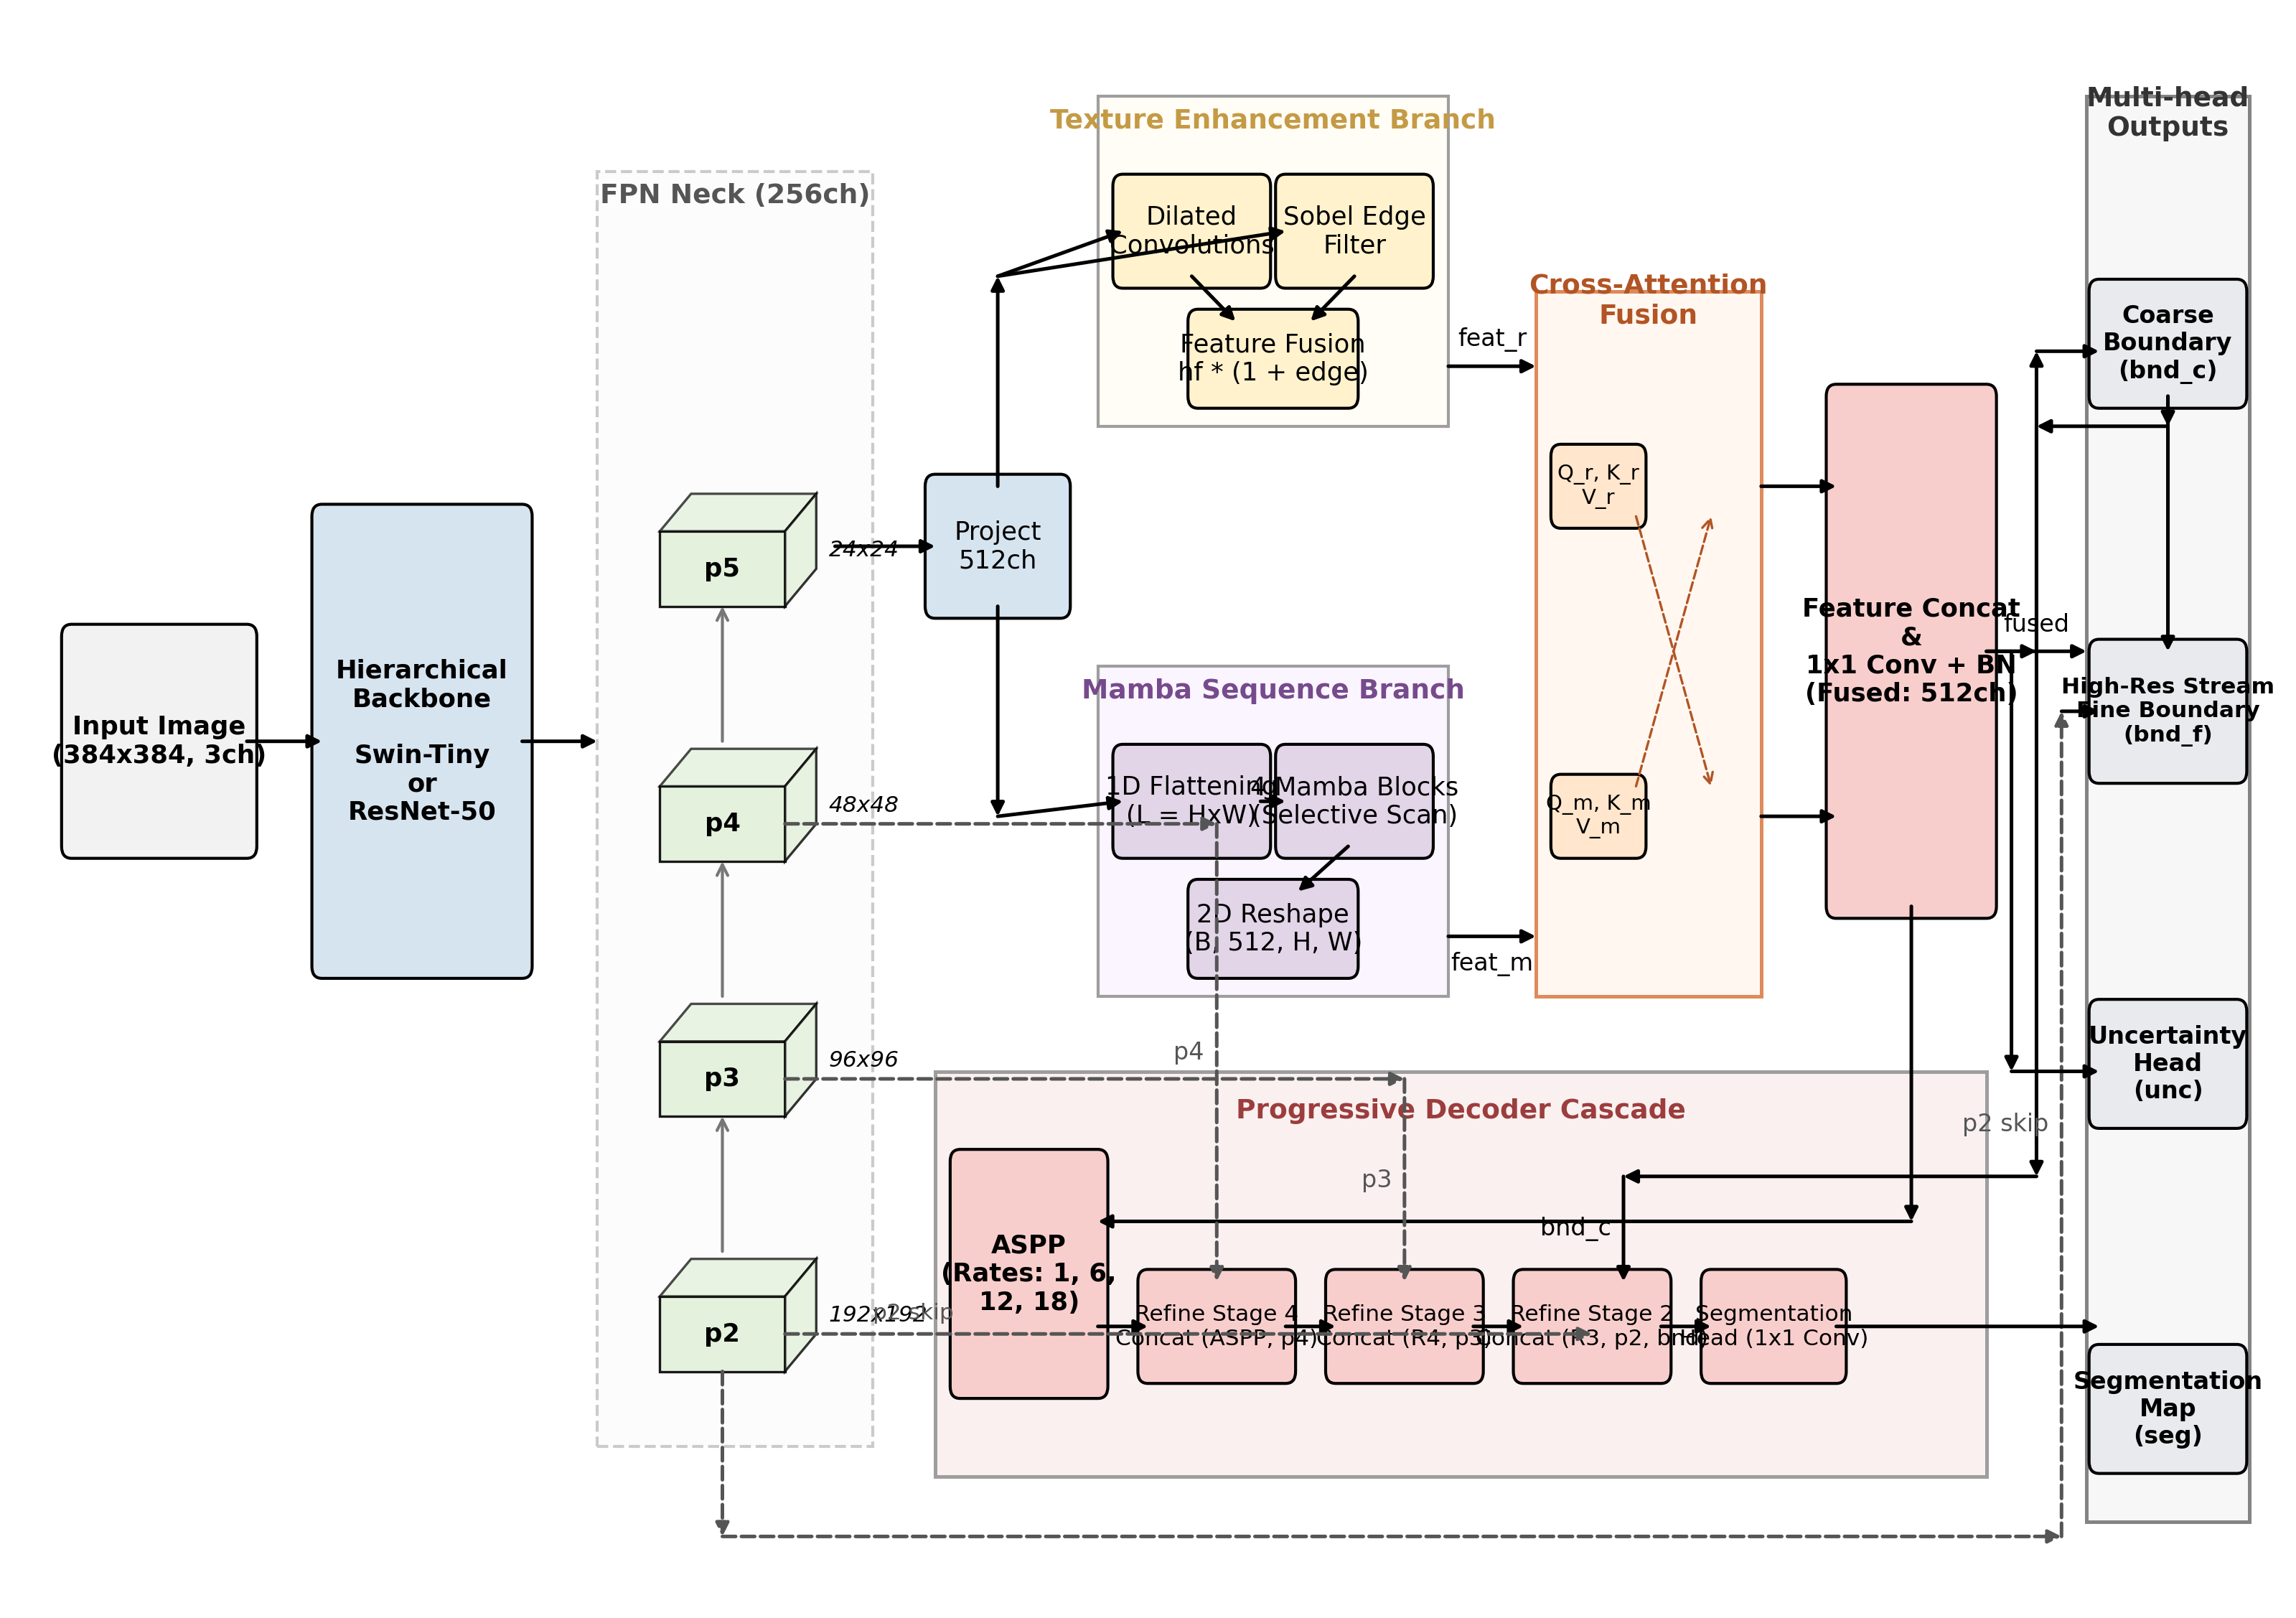
\includegraphics[width=\linewidth]{main2fig/fig7_architecture_schematic.png}
  \caption{Architecture overview of the three configurations evaluated in this study. All models share the same FPN neck, loss function, and decoder structure. The only differences are the backbone (ResNet-50 vs.\ Swin-Tiny) and the sequence modeling branch (Transformer vs.\ Mamba). Swin+Mamba additionally includes a cross-attention fusion module between the two branches.}
  \label{fig:arch}
\end{figure}
% ─────────────────────────────────────────────────────────────────────────────

\subsection{Evaluation Metrics}
Model performance is measured using four metrics, computed identically for all three models via a shared evaluation class. Structure Measure (Sm)~\cite{fan2017structure} evaluates object-level and region-level structural similarity between the predicted map and the ground truth. Enhanced-alignment Measure (Em)~\cite{fan2021metrics} captures pixel-level and image-level alignment jointly; we report both the mean and max over a 255-threshold sweep. Weighted F-measure (wFm) computes precision and recall with boundary-proximity weights derived from distance transforms, down-weighting pixels far from the object edge. Mean Absolute Error (MAE) measures per-pixel absolute deviation between the predicted probability map and the binary ground truth. For all metrics except MAE, higher is better.

Crucially, while the COD10K test set comprises 4,000 images in total, 1,974 of these are non-camouflaged (NonCAM) negative control samples that contain no target objects (i.e., empty ground-truth masks). In line with the standard evaluation protocol established in the COD literature (e.g.,~\cite{fan2020cod,fan2022sinetv2}), we compute all quantitative metrics exclusively over the 2,026 camouflaged (CAM) test images. Evaluating models over the entire 4,000-image set would artificially deflate weighted F-measure and inflate S-measure metrics due to the presence of empty ground-truth masks.


% ─────────────────────────────────────────────────────────────────────────────
\section{Results and Discussion}
\label{result}
% ─────────────────────────────────────────────────────────────────────────────

The controlled setup described in Section~III produces clean, directly comparable numbers across all three models. Every difference in the results traces back to architecture alone , nothing else changed between runs.

\subsection{Quantitative Results}

Table~\ref{tab:results} summarizes the best checkpoint performance for each model on the COD10K test set.

\begin{table}[t]
\centering
\caption{Best checkpoint results on COD10K test set. All models trained for 100 epochs under identical conditions. Bold indicates best performance per metric.}
\label{tab:results}

\resizebox{\columnwidth}{!}{%
\begin{tabular}{lcccccc}
\toprule
\textbf{Model} & \textbf{S$_m$} & \textbf{E$_m$\,(mean)} & \textbf{E$_m$\,(max)} & \textbf{wF$_m$} & \textbf{MAE} & \textbf{Params} \\
\midrule
ResNet + Transformer & 0.8045 & 0.8348 & 0.9479 & 0.6268 & 0.0435 & 49.3M \\
ResNet + Mamba       & 0.8097 & 0.8387 & 0.9454 & 0.6408 & 0.0424 & 62.6M \\
Swin + Mamba         & \textbf{0.8401} & \textbf{0.8742} & \textbf{0.9496} & \textbf{0.6979} & \textbf{0.0341} & 67.2M \\
\bottomrule
\end{tabular}%
}
\end{table}

Fig.~\ref{fig:bar} summarizes the best checkpoint results visually. The Sm and wFm bars make the ranking unambiguous , Swin+Mamba leads on both by a margin that is visible even at this scale. The MAE panel on the right tells the cleaner story: Swin+Mamba's bar is noticeably shorter than the two ResNet models, which sit at nearly the same height as each other. This reinforces the main finding , the backbone swap produced a qualitatively different result, the decoder swap did not.

% ── Bar chart figure ─────────────────────────────────────────────────────────
\begin{figure}[t]
  \centering
  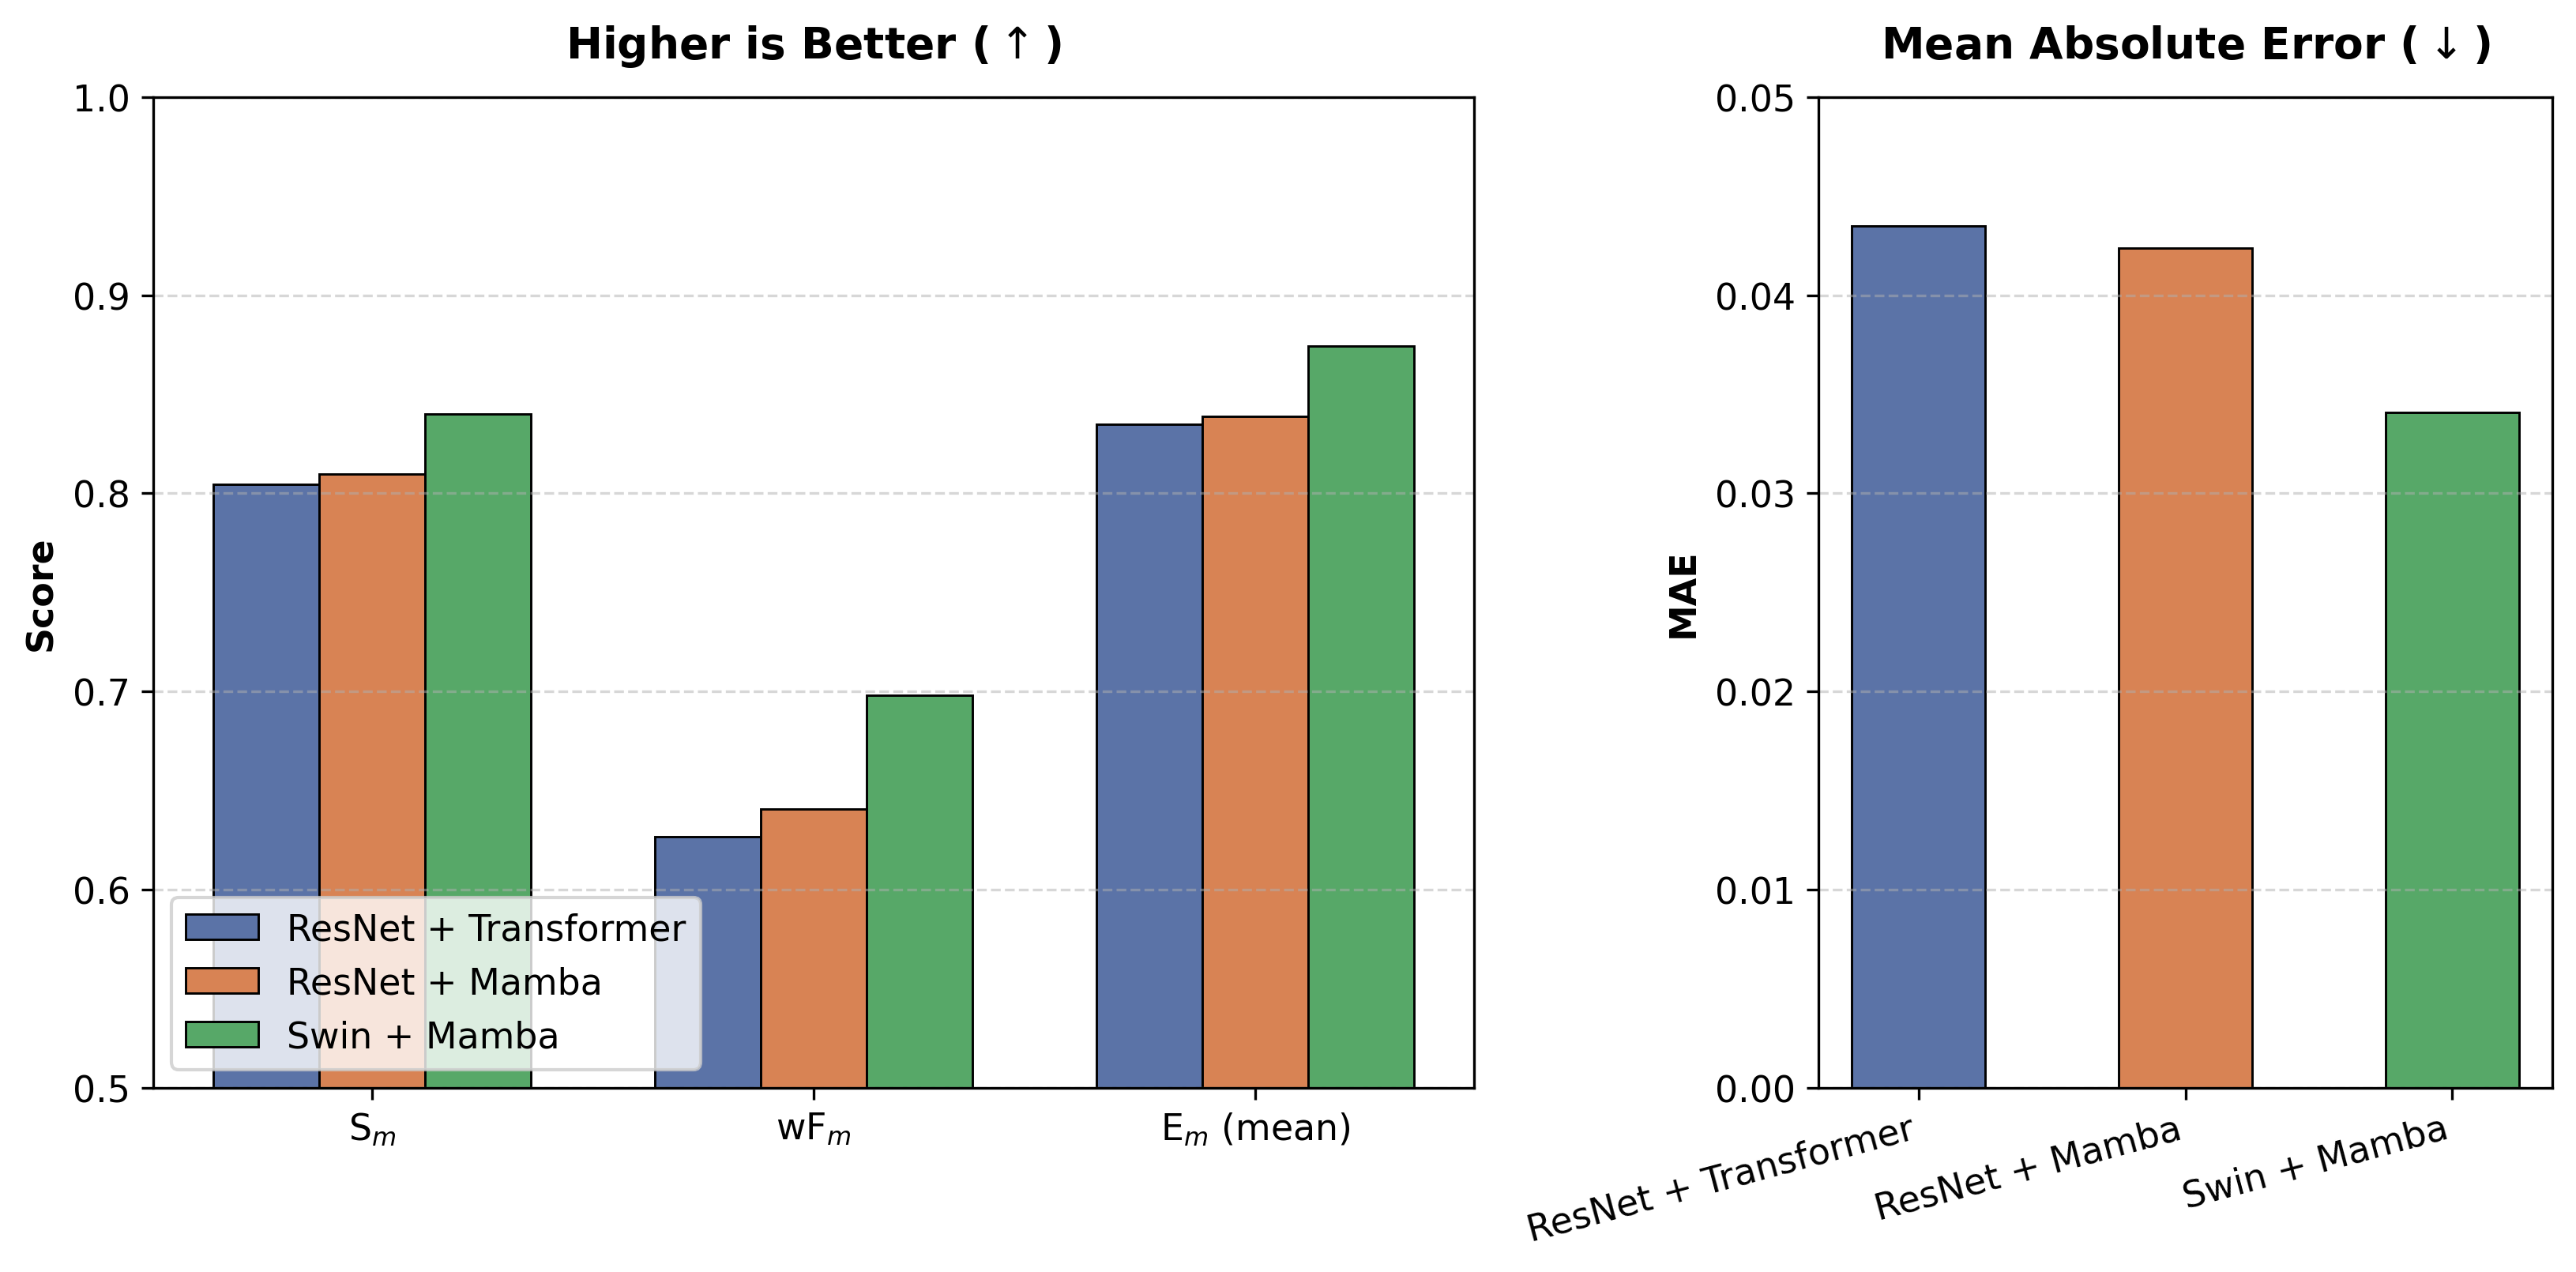
\includegraphics[width=\linewidth]{main2fig/fig5_best_checkpoint_bar.png}
  \caption{Best checkpoint performance on the COD10K test set. Left: Sm, wFm, and Em\,(mean), where higher is better. Right: MAE, where lower is better. The backbone upgrade from ResNet-50 to Swin-Tiny (ResNet+Mamba $\to$ Swin+Mamba) produces a visibly larger improvement than the decoder swap (ResNet+Transformer $\to$ ResNet+Mamba).}
  \label{fig:bar}
\end{figure}
% ─────────────────────────────────────────────────────────────────────────────

Swin+Mamba is the clear winner on Sm, wFm, and MAE , the three metrics that most directly measure segmentation quality and boundary precision. ResNet+Mamba edges out ResNet+Transformer on Sm (0.8097 vs.\ 0.8045) and wFm (0.6408 vs.\ 0.6268), but the gap between the two ResNet models is much smaller than the gap between either ResNet model and Swin+Mamba. The MAE gap is particularly telling: Swin+Mamba reaches 0.0341 against ResNet+Transformer's 0.0435 , a 22\% reduction in per-pixel error.

The E$_m$ numbers follow a similar pattern. Swin+Mamba achieves the highest E$_m$\,(max) of 0.9496, outperforming ResNet+Transformer (0.9479) and ResNet+Mamba (0.9454). On E$_m$\,(mean), Swin+Mamba leads with 0.8742 compared to ResNet+Mamba's 0.8387 and ResNet+Transformer's 0.8348. This consistent outperformance across both mean and max E$_m$ metrics indicates that the Swin-based architecture produces significantly better pixel-level alignment across various decision thresholds.

\subsection{Training Dynamics}
The training logs reveal as much as the final numbers. All three models start from a similar position , Sm around 0.58--0.60 at epoch 5 , and diverge through the first 30 epochs.

ResNet+Transformer is the slowest to take off. At epoch 10 it sits at Sm = 0.7300, slightly below ResNet+Mamba's 0.7310. By epoch 15 it reaches 0.7700, still trailing ResNet+Mamba's 0.7750. The gap narrows through mid-training, and by epoch 35 ResNet+Transformer briefly surges to Sm = 0.8010 against ResNet+Mamba's 0.7980 at epoch 34. After that both models plateau. ResNet+Transformer's best checkpoint (0.8045) is reached at epoch 56, and the model effectively stops improving , the last 44 epochs produce no further gains, with Sm oscillating in the 0.800--0.803 band.

ResNet+Mamba follows a similar plateau pattern but with more volatility. Its best Sm of 0.8097 arrives at epoch 55, and the remaining epochs hover around 0.803--0.809 without meaningful improvement. The loss continues rising after epoch 55 , from around 1.68 at the best checkpoint to 1.99 by epoch 100 , suggesting the model has converged and is beginning to drift slightly. That rising test loss with flat Sm is a mild sign of overfitting in the boundary terms rather than the segmentation head.

Swin+Mamba converges faster and keeps improving longer. It hits Sm = 0.8150 by epoch 22, already above where the ResNet models plateau. By epoch 32 it is at 0.8350, a level neither ResNet model ever reaches. It continues making incremental gains through epoch 75, where it records its best Sm of 0.8401. After that it also plateaus, though at a higher level , Sm stays in the 0.837--0.839 range through epoch 100.

One practical note on training time: Swin+Mamba completed 100 epochs in 13\,h\,52\,min, ResNet+Transformer in 14\,h\,39\,min, and ResNet+Mamba in 15\,h\,25\,min. Mamba's linear-time sequence modeling gives it a wall-clock advantage over the Transformer even at $384{\times}384$ resolution.

\subsection{Effect of Backbone vs.\ Decoder Choice}

The two controlled comparisons at the heart of this paper are straightforward to read from Table~\ref{tab:results}. Fig.~\ref{fig:gain} makes this decomposition concrete , the backbone gain bar (red) is visibly taller than the decoder gain bar (purple) on both Sm and wFm.

% ── Gain decomposition figure ────────────────────────────────────────────────
\begin{figure}[t]
  \centering
  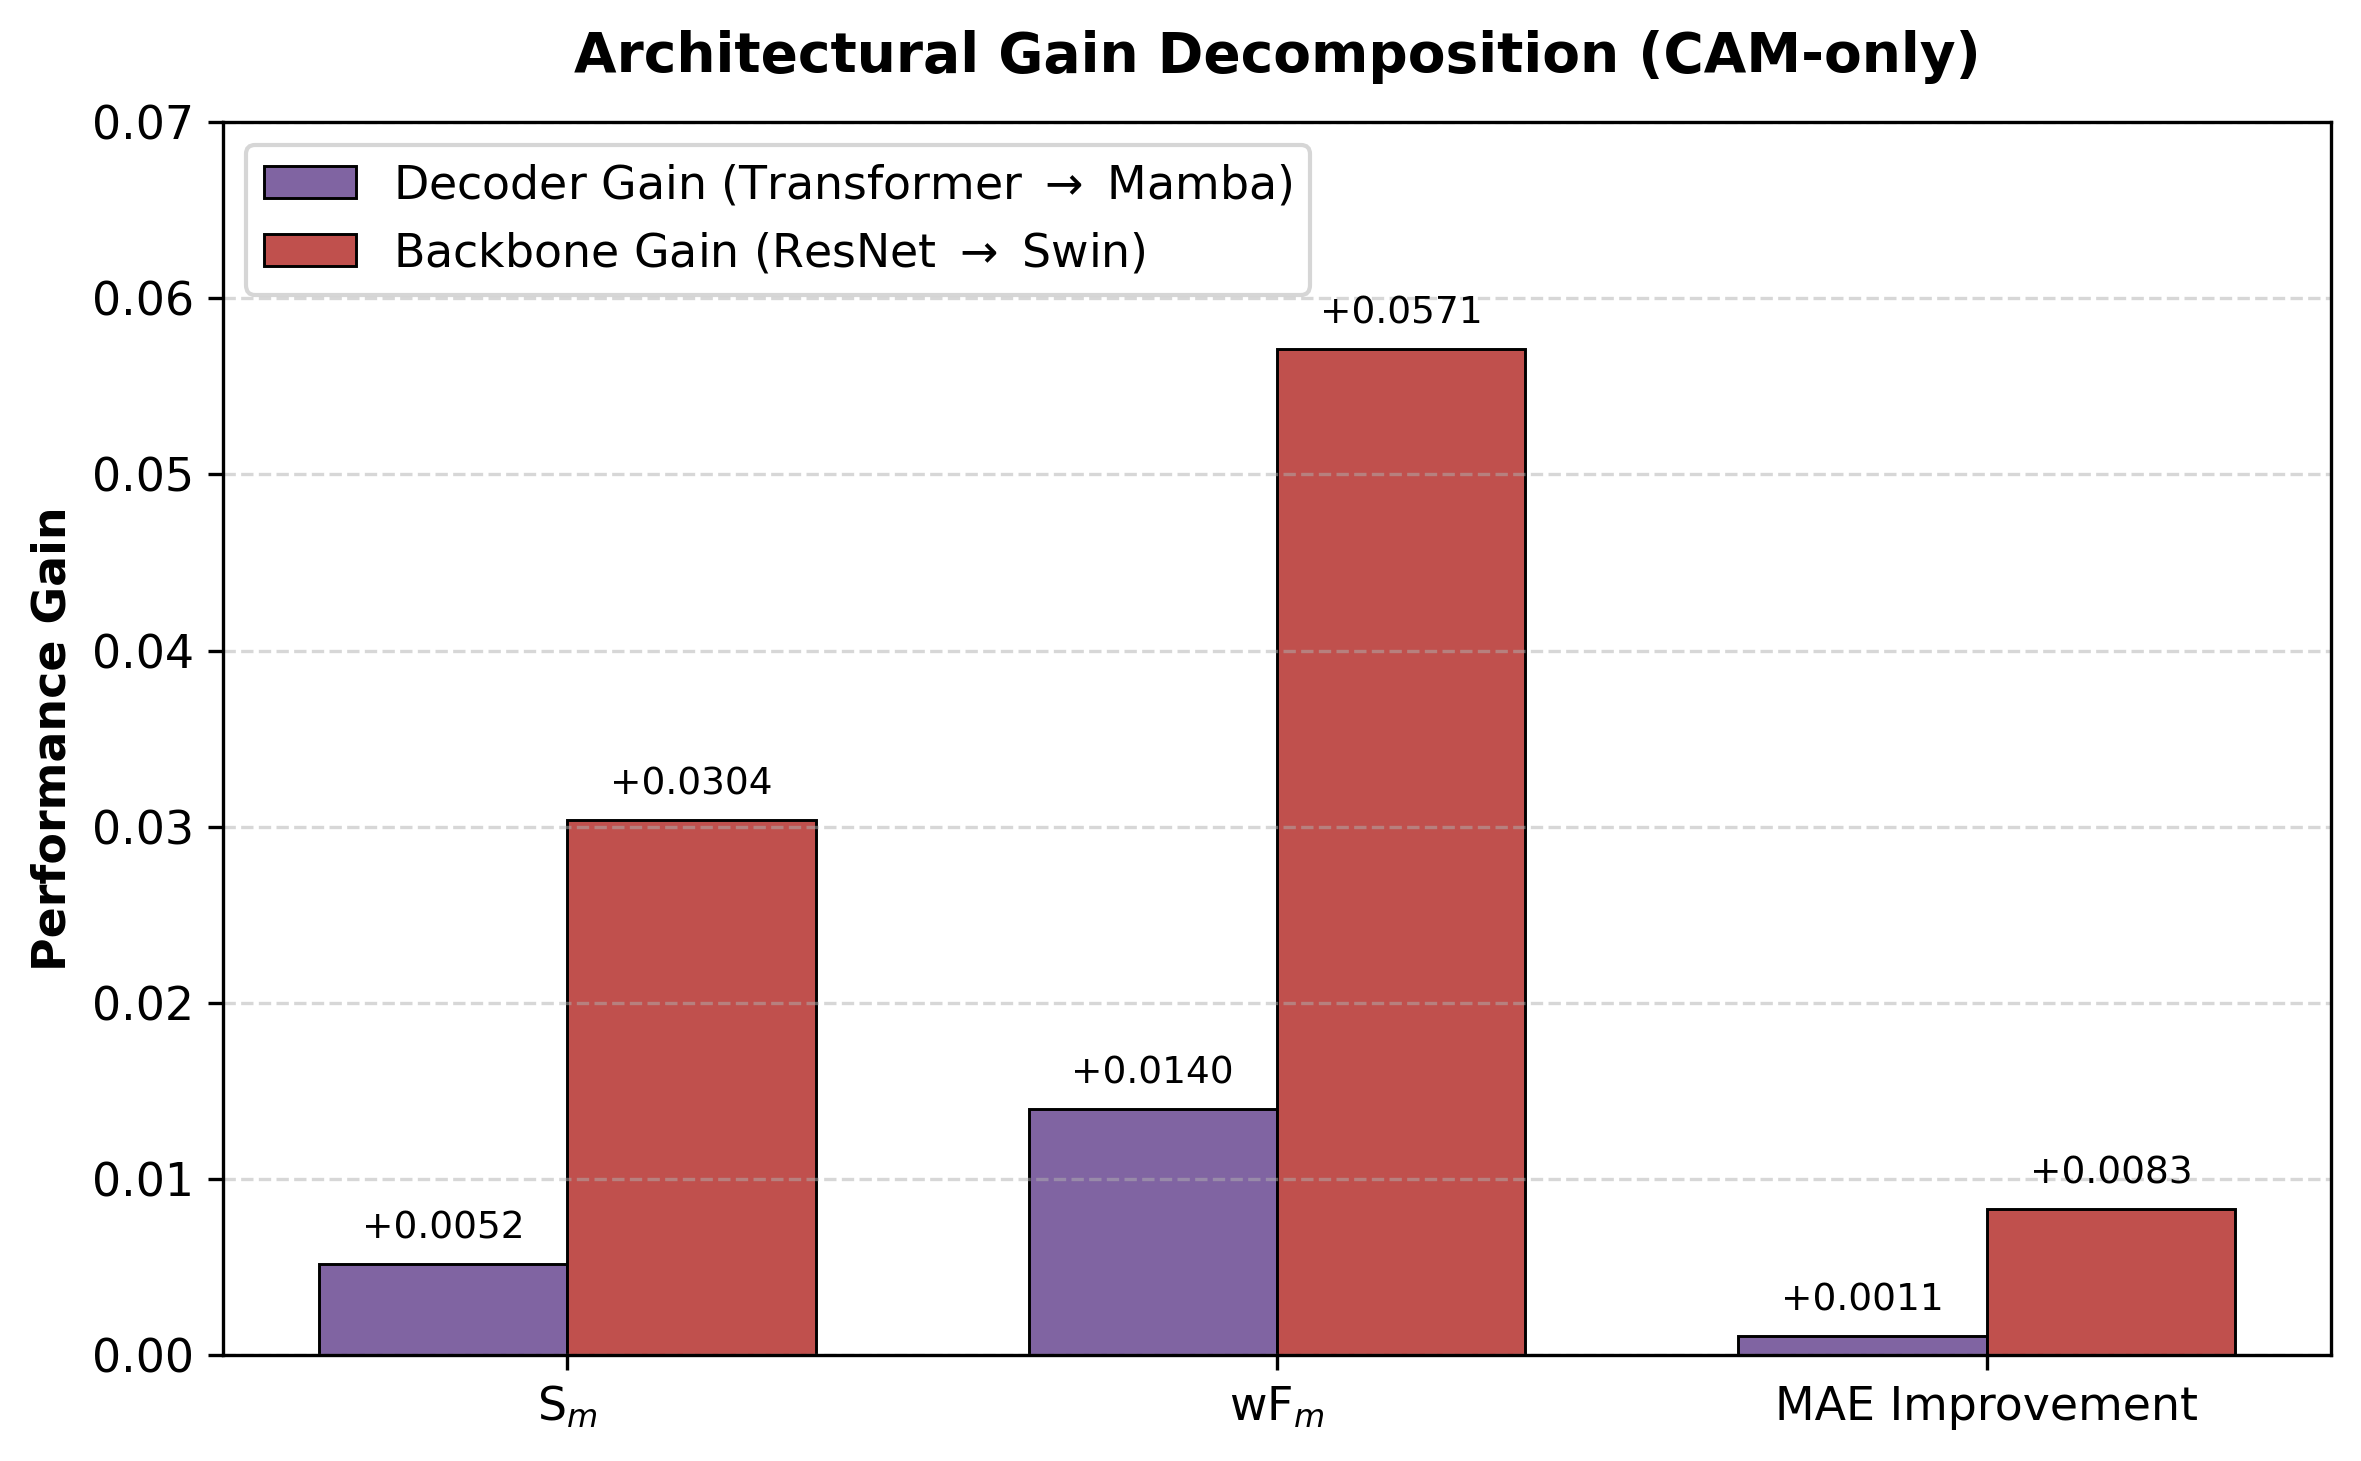
\includegraphics[width=\linewidth]{main2fig/fig6_gain_decomposition.png}
  \caption{Isolated architectural contributions under matched training conditions. Purple bars show the gain from swapping the Transformer decoder for Mamba on a fixed ResNet-50 backbone. Red bars show the gain from swapping the ResNet-50 backbone for Swin-Tiny on a fixed Mamba decoder. The backbone gain dominates across all metrics. Both the decoder swap and the backbone swap contribute to reducing Mean Absolute Error (MAE).}
  \label{fig:gain}
\end{figure}
% ─────────────────────────────────────────────────────────────────────────────

\paragraph{\textbf{Decoder choice, backbone held constant.}} Swapping the Transformer decoder for Mamba on a ResNet-50 backbone raises Sm from 0.8045 to 0.8097, wFm from 0.6268 to 0.6408, and Em\,(mean) from 0.8348 to 0.8387. MAE also improves slightly (0.0424 vs.\ 0.0435). The gain is real but modest. Under the same training conditions and backbone, Mamba holds a consistent edge over Transformer as a sequence decoder.

\paragraph{\textbf{Backbone choice, decoder held constant.}} Swapping ResNet-50 for Swin-Tiny while keeping Mamba as the decoder raises Sm from 0.8097 to 0.8401, wFm from 0.6408 to 0.6979, and MAE from 0.0424 to 0.0341. Every metric moves substantially. The Swin backbone gain (0.0304 Sm) is roughly six times larger than the Mamba decoder gain over Transformer (0.0052 Sm). The MAE column is particularly revealing: swapping the Transformer decoder for Mamba improves MAE by 0.0011, while the backbone swap then recovers and exceeds both, cutting MAE by 0.0083. The conclusion is hard to avoid: backbone hierarchy matters more than decoder sophistication.

This does not mean decoder choice is irrelevant , the Mamba advantage on wFm and Em\,(max) is consistent and meaningful, particularly for boundary sharpness. But if forced to choose where to invest model capacity first, the backbone is the more leveraged decision.

\subsection{Failure Cases and Limitations}

The training logs and qualitative outputs together point to several systematic failure patterns that the numbers alone do not fully capture.

\paragraph{\textbf{Qualitative predictions on camouflaged samples.}} Fig.~\ref{fig:qualcam} shows predictions from all three models on five camouflaged test images from COD10K. Several patterns are immediately visible. On sample 3304 (butterfly on leaves), all three models correctly localize the object body but miss the thin antennae , these fall below the effective resolution of the boundary supervision at $384{\times}384$. On sample 1010 (scorpionfish on coral), the ResNet models produce slightly over-segmented blobs while Swin+Mamba recovers a tighter boundary, consistent with its lower MAE. Sample 521 (sea slug) is the most instructive failure: ResNet+Mamba and ResNet+Transformer both find the elongated body of the slug, but Swin+Mamba additionally hallucinates a large false-positive region on the right side of the frame, suggesting the cross-attention fusion module occasionally amplifies texture responses in highly cluttered backgrounds. Sample 3804 (moth on gravel) shows all three models succeeding on the body but losing the thin leg and antenna structures. Sample 1434 (cat on rug) is the easiest case , all three produce clean, accurate masks with minor boundary disagreements.

% ── Camouflaged qualitative figure ───────────────────────────────────────────
\begin{figure}[t]
  \centering
  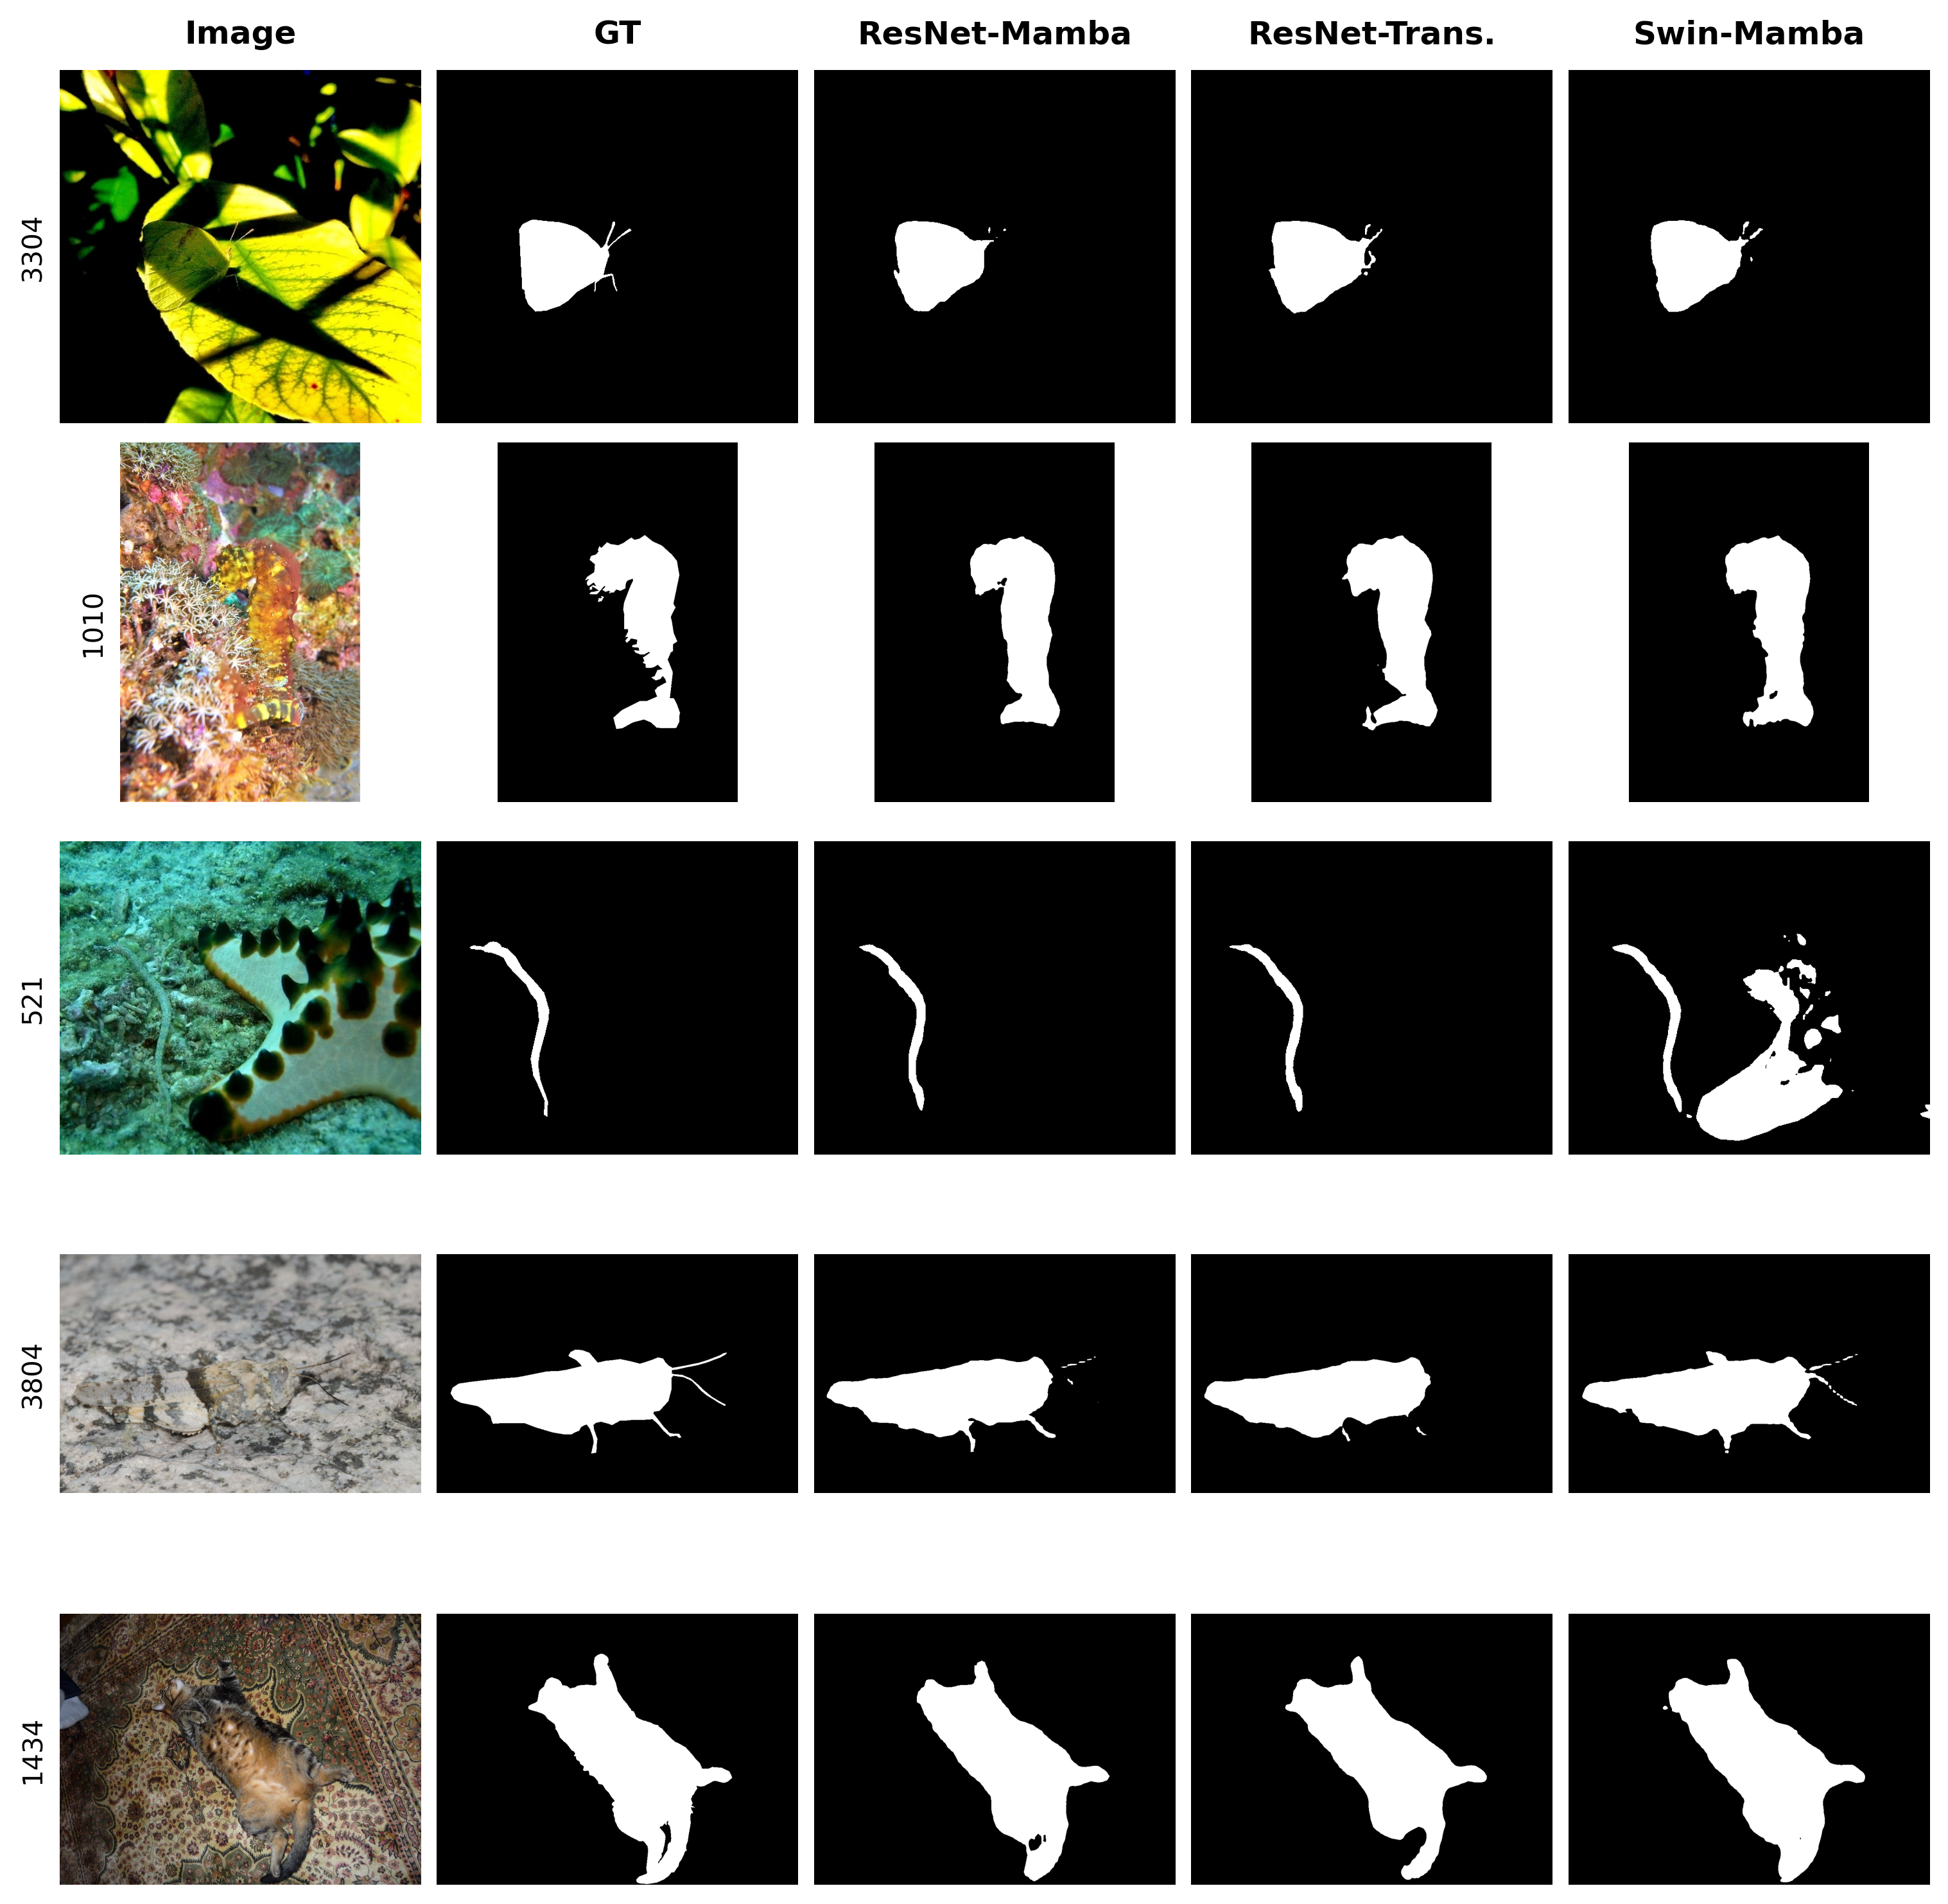
\includegraphics[width=\linewidth]{main2fig/comparison_CAM.png}
  \caption{Qualitative predictions on five camouflaged samples from the COD10K test set. Columns show the input image, ground truth (GT) mask, and predictions from ResNet+Mamba, ResNet+Transformer, and Swin+Mamba respectively. Row IDs correspond to COD10K image indices. All models handle compact object bodies reasonably well. Thin structures (antennae, legs) and cluttered backgrounds (sample 521) remain challenging across all three configurations.}
  \label{fig:qualcam}
\end{figure}
% ─────────────────────────────────────────────────────────────────────────────

\paragraph{\textbf{Non-camouflaged samples.}} Fig.~\ref{fig:qualnoncam} shows predictions on five samples from the non-camouflaged portion of the test split , images where the ground-truth mask is empty. All three models output entirely black predictions, meaning all three correctly suppress false positives on these negative examples. While this reflects correct behavior on the COD10K benchmark, it also means none of the models would generalize gracefully to a deployment scenario where non-camouflaged objects need to be detected alongside camouflaged ones. The models have learned to be conservative by default, which serves the benchmark but would be a limitation in any real-world system.

% ── Non-camouflaged qualitative figure ───────────────────────────────────────
\begin{figure}[t]
  \centering
  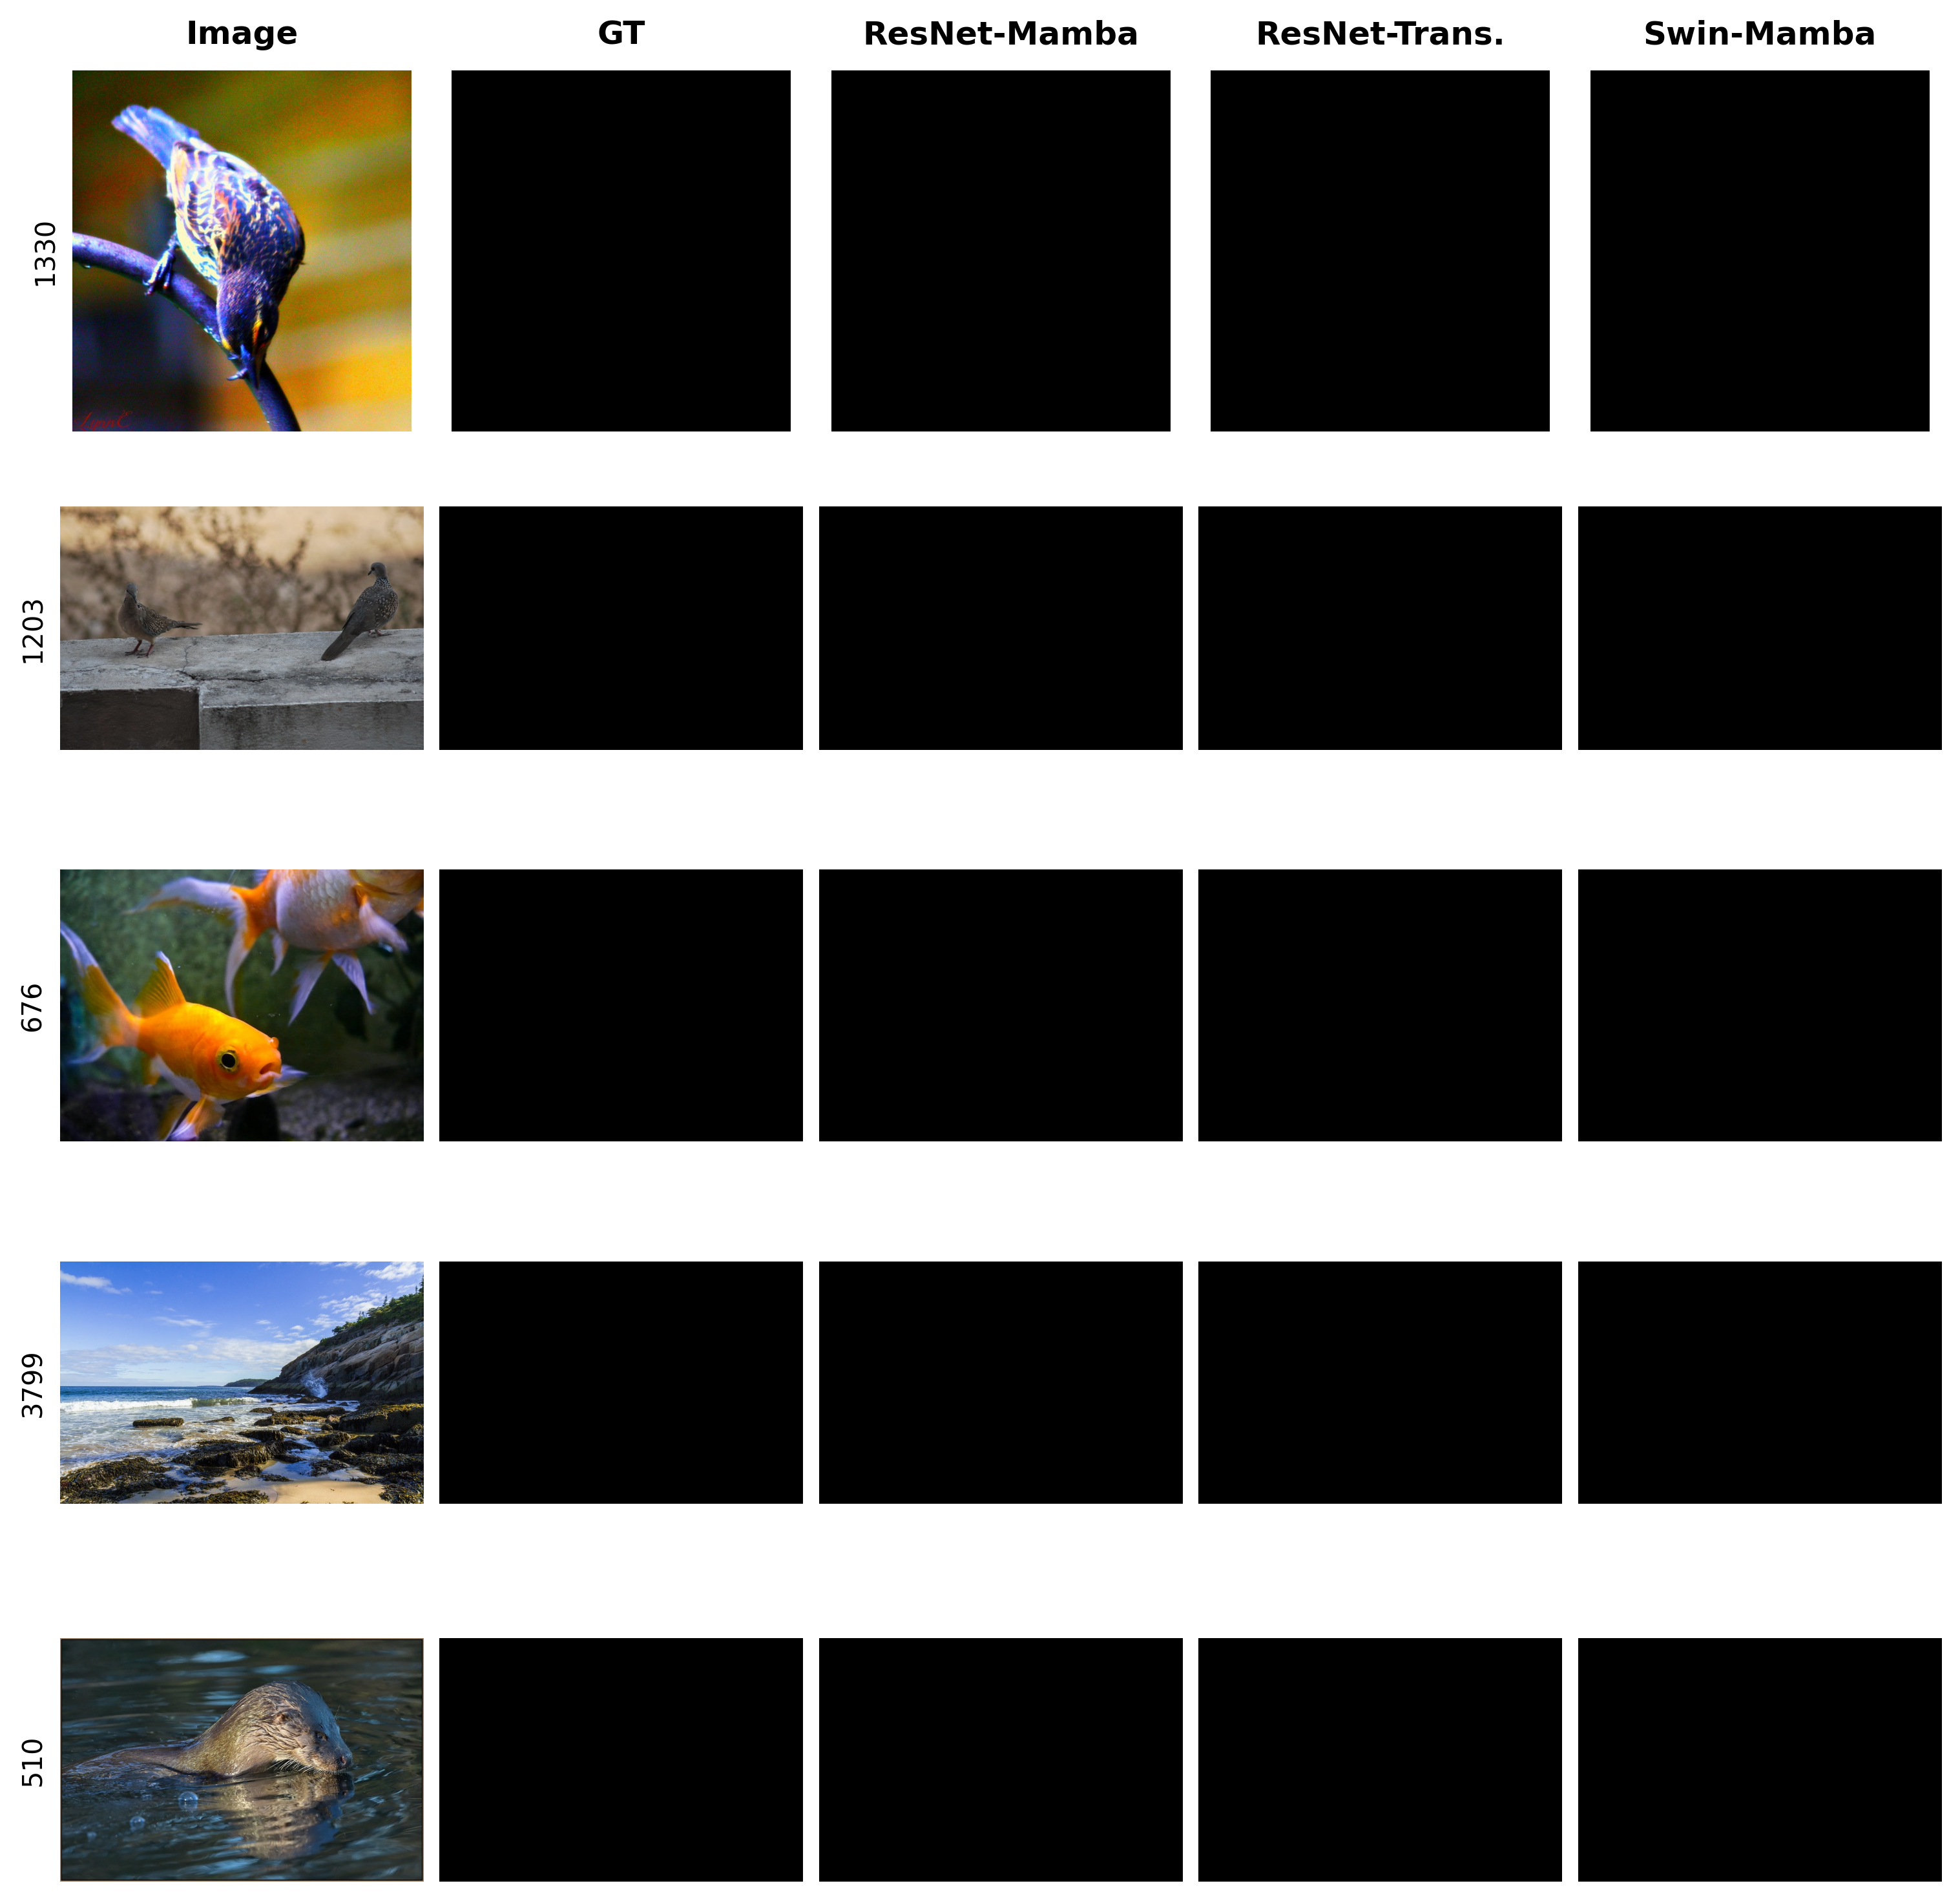
\includegraphics[width=\linewidth]{main2fig/comparison_NonCAM.png}
  \caption{Predictions on five non-camouflaged samples (empty ground-truth masks). All three models correctly output blank predictions, indicating no false positives on these examples. While this reflects correct benchmark behavior, it reveals that the models are calibrated toward suppression by default, which would limit performance in mixed detection settings.}
  \label{fig:qualnoncam}
\end{figure}
% ─────────────────────────────────────────────────────────────────────────────

\paragraph{\textbf{Early training instability at high learning rates.}} All three models show loss spikes during epochs 1--5, when the learning rate is ramping up through the warmup phase. The bnd and bnd\_c loss components drive large gradients early, and the gradient clip at 2.0 is doing real work in the first few epochs. A more conservative boundary weight during warmup would likely smooth this out.

\paragraph{\textbf{Plateau without recovery.}} Both ResNet models stop improving before epoch 60 and show no further gains for the remaining 40+ epochs. This is not because they have reached their theoretical ceiling , Swin+Mamba is still improving at epoch 60, using the same decoder. The plateau is a backbone problem. Once ResNet-50 features are saturated, the decoder cannot compensate. This suggests that for longer training runs or larger datasets, ResNet-50 would be the bottleneck.

\paragraph{\textbf{Boundary sharpness vs.\ structural accuracy tradeoff.}} Under a fixed ResNet-50 backbone, the Transformer decoder achieves a slightly higher $E_m$\,(max) than Mamba (0.9479 vs.\ 0.9454), whereas Mamba leads on $E_m$\,(mean) and $wF_m$. This indicates that while the Transformer model can produce very clean binary masks at one specific optimal threshold, Mamba offers consistently better alignment and weighted boundary precision on average. Swin+Mamba, by contrast, benefits from the hierarchical backbone to achieve the highest performance across all metrics, including $E_m$\,(max) at 0.9496.

\paragraph{\textbf{Mamba's sequential scan on 2D spatial data.}} The Mamba branch processes the 2D feature map by flattening it to a 1D sequence before applying the selective scan. This imposes a fixed scan ordering on what is fundamentally a 2D spatial structure. For camouflaged objects elongated along the scan direction (row-major), the SSM has an easier time modeling their extent than for objects oriented perpendicular to the scan. This is visible in the Em\,(max) numbers , the Transformer, which has no ordering bias, performs better at the single best threshold while Mamba does better on average. Bidirectional or 2D scan strategies would likely close this gap.

\paragraph{\textbf{Objects with no discriminating signal.}} All three models struggle, by design, with objects that are genuinely indistinguishable from their background in color, texture, and edge profile. The boundary loss not converging below a certain floor , around 0.09--0.10 for the fine boundary head across all models , indicates that some fraction of the test set simply does not have recoverable boundary information at this resolution. No architectural change addresses this; it is a fundamental property of the hardest COD examples.

\subsection{Discussion}
Two conclusions come clearly from these results. First, under matched training conditions, Mamba outperforms a standard Transformer decoder on the same backbone. The advantage is not large , 0.0052 Sm , but it is consistent across all metrics that measure spatial and boundary quality, and it comes with a wall-clock speed advantage from linear-time sequence modeling. Second, the backbone is the dominant factor. The Swin backbone gain is an order of magnitude larger than the decoder gain, which means that COD papers reporting improvements from new decoder designs while also upgrading the backbone are almost certainly attributing the backbone gain to the decoder.

The broader implication is that controlled comparisons of the kind we run here should be standard practice in COD, not the exception. The literature has accumulated a large number of results that cannot be meaningfully compared to each other because training conditions were never matched. Any paper that changes the backbone, the loss, the schedule, and the decoder simultaneously cannot tell you which of those changes mattered. We hope the matched baseline provided here gives the community a fixed reference point that future decoder-focused work can be evaluated against fairly.


% ─────────────────────────────────────────────────────────────────────────────
\section{Conclusion}
\label{con}
% ─────────────────────────────────────────────────────────────────────────────

This paper set out to answer a specific question: when you control for everything except the architecture, how much do backbone and decoder choice actually matter for camouflaged object detection? The answer, based on 100 epochs of matched training across three configurations on COD10K, is that backbone choice matters substantially more than decoder choice, and that Mamba holds a consistent edge over Transformer as a decoder when the backbone is held fixed.

The numbers are clear enough on their own. Swapping a Transformer decoder for Mamba on a ResNet-50 backbone improves Sm by 0.0052 and wFm by 1.4 percentage points. Swapping the ResNet-50 backbone for Swin-Tiny while keeping Mamba improves Sm by 0.0304 and cuts MAE by 20\%. The backbone gap is roughly six times the decoder gap. Both are real effects, but they are not close in magnitude.

What makes these results useful beyond the specific numbers is the setup that produced them. All three models trained under exactly the same optimizer, schedule, loss, resolution, augmentation pipeline, random seed, and hardware. The differences in the table trace back to architecture and nothing else. That kind of clean attribution is rare in the COD literature, where most published comparisons mix backbone upgrades, new training recipes, and new decoder designs simultaneously and then report a single combined number.

There are honest limitations here too. We test one backbone per family , ResNet-50 for CNNs, Swin-Tiny for hierarchical Transformers , and one decoder depth for each sequence modeling approach. A larger ResNet or a deeper Mamba stack might shift the relative gaps. We also train on COD10K alone, without pretraining on salient object detection datasets or using additional supervision signals, which is a deliberate choice for fairness but leaves performance below what specialized models with richer training pipelines achieve. The qualitative failure analysis in Section~IV points to structural limitations , Mamba's 1D scan ordering on 2D spatial data, ResNet-50's saturation plateau, and the irreducible difficulty of objects with no recoverable boundary signal , that architectural novelty alone will not resolve.

The practical takeaway for future work is straightforward. If the goal is a better COD model, invest in the backbone first. A stronger hierarchical backbone with richer multi-scale representations gives the decoder more to work with, and as our results show, the decoder cannot compensate for weak backbone features regardless of how sophisticated it is. Once the backbone is fixed, Mamba is the better decoder choice over a standard Transformer under the conditions we tested , faster to train, better on boundary metrics, and competitive or superior on structural accuracy. Future work comparing decoder architectures should anchor those comparisons to a fixed strong backbone and report results with matched training conditions if they want the comparison to mean anything.


\bibliographystyle{IEEEtranN}
\bibliography{refer}

\end{document}